%!TEX root = ../MasterThesis.tex

\chapter{Context Analysis} % (fold)
\label{cha:context_analysis}

This chapter looks into the scenario of \gls{E-commerce} fraud investigation in detail. It starts with an in-depth description of the \gls{E-commerce} scenario followed by an analysis of the stakeholders involved. It further describes the kind of information each stakeholder has in their local context, and their objectives to take part on the information sharing and collaboration initiative. Based on the analysis of the possible kinds of \gls{E-commerce} fraud incidents and the current process of their investigation, the chapter closes with a description of the specific scenario, that has been selected for this Master thesis.

% sub chapter scenario description
%!TEX root = ../MasterThesis.tex

\section{E-commerce Scenario}
\label{sec:e_commerce_scenario}

\textbf{E-commerce} as a term relates to the trading of products or services utilizing a computer network such as the Internet. It is usually categorized into the following four different subfields \citep{sen2015study}:\@

\begin{enumerate}
  \item \textbf{Business-To-Business (\gls{B2B})}: refers to electronic trading between companies with the objective to improve their supply chain processes
  \item \textbf{Business-To-Consumer (\gls{B2C})}: refers to electronic trading between a company and it's consumers (most publicly known example for it is Amazon.com)
  \item \textbf{Consumer-To-Consumer (\gls{C2C})}: refers to electronic trading between consumers (most publicly known example for that is eBay)
  \item \textbf{Consumer-To-Business (\gls{C2B})}: referes to electronic trading between consumers and businesses (most publicly known example for this is TaskRabbit)
\end{enumerate}

This Master thesis will \textbf{\underline{solely}} focus on the \textbf{\gls{B2C}} aspect of E-commerce. In that case a \textbf{consumer} is using an \textbf{E-commerce shop} of a \textbf{merchant} on the Internet to order products or services online. The merchant is offering a catalog of available products or services on the Web, that is available and accessible by the general public and usually has an at least nation-wide if not global reach. The merchant can either run the E-commerce shop software on her own servers (on-premise) or can outsource this additional sales channel to a 3$^{rd}$ party hosting company or \textbf{cloud service provider (\gls{CSP})}. Also the E-commerce shop software itself can either be developed by the merchant in-house or acquired as a boxed product from an \textbf{Independent Software Vendor (\gls{ISV})} on the market. For business accounting purposes the merchant also runs a bank account with the \textbf{acquirer} (see Figure~\ref{fig:images_ecommerce_scenario}). \\

When placing an order with the merchant online the consumer is normally using a \textbf{credit card} for finalizing the transaction. This credit card has originally been handed out by the \textbf{issuing bank} to the consumer. Additionally some online shops make it mandatory for the consumer to create an user account with them while others do not. The former is the preferred way when consumers are repetitively buying from that merchant, whereas the latter might be used for one-time or irregular shopping trips online. To be able to connect to the Internet the consumer also relies on a service of an \textbf{Internet Service Provider (\gls{ISP})}. The whole initial setup for participating on E-commerce activities is found in Figure~\ref{fig:images_ecommerce_scenario}.\@

\begin{figure}[H]
	\centering
		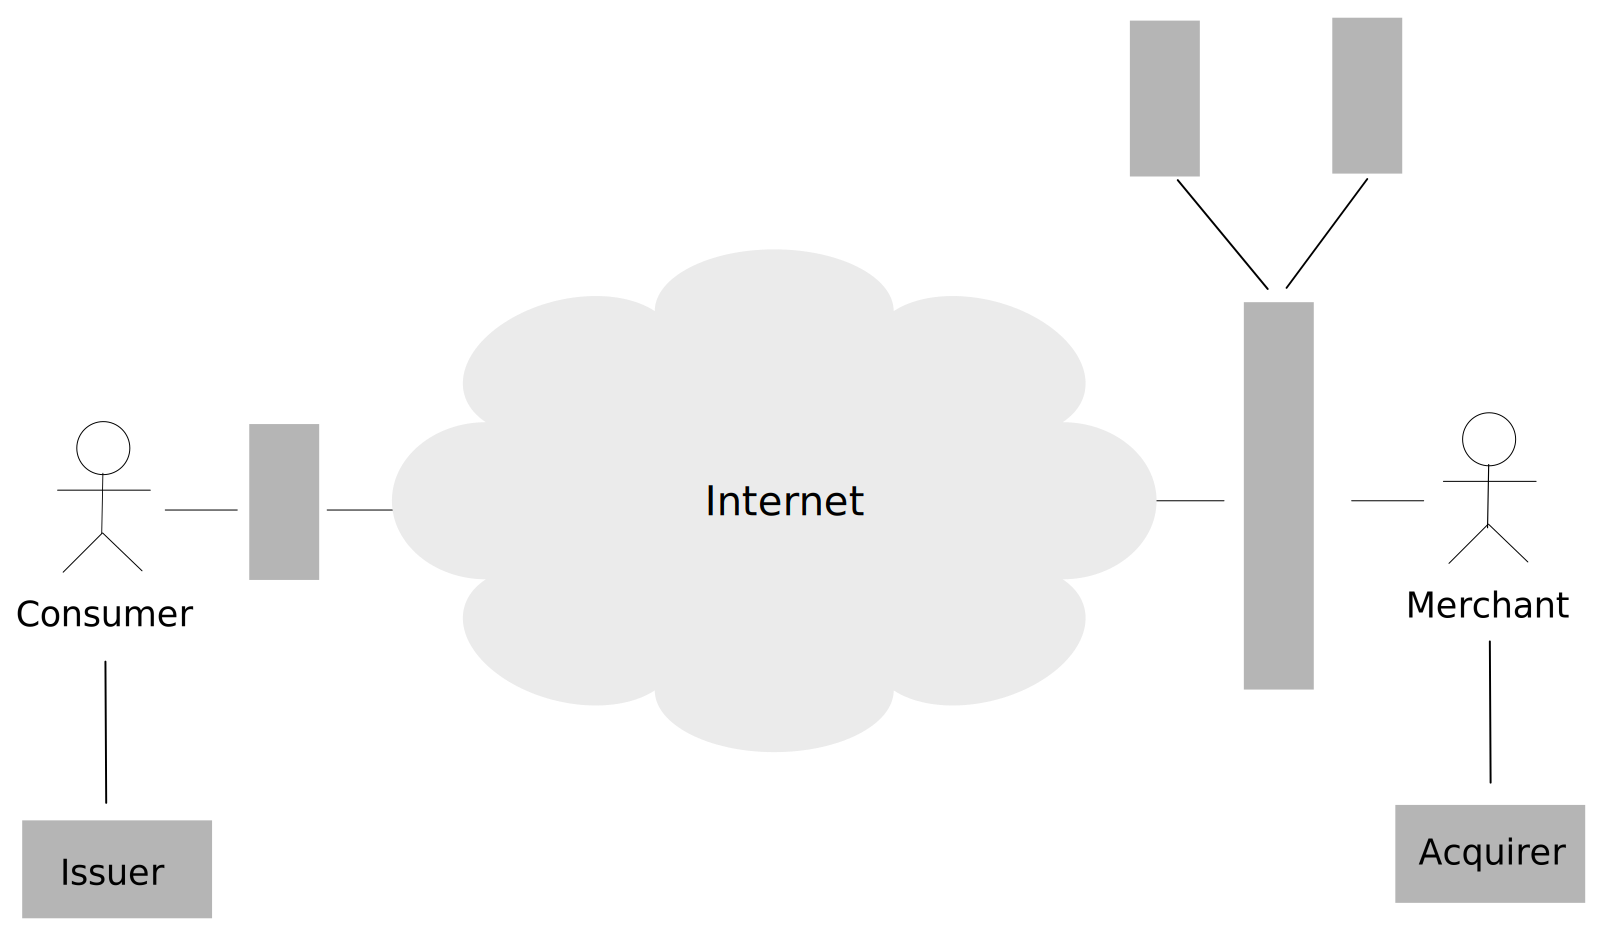
\includegraphics[width=0.8\columnwidth]{images/e-commerce-scenario.pdf}
	\caption{E-commerce Fundamentals}
\label{fig:images_ecommerce_scenario}
\end{figure}

When the consumer places the \textbf{order} online, the merchant receives at least a \textbf{list of products or services} from the current shopping cart of the consumer, the \textbf{identification} of the consumer as well as the \textbf{delivery address} to ship the physical items to. If the transaction is going to be finalized with a credit card, the consumer will have to provide additional information like her \textbf{billing address} and \textbf{credit card information} (including the credit card number, the expiry date and the security number of the card). \\

The merchant usually does not validate the credit card information on her own. For that purpose she is relying on another 3$^{rd}$ party service offered on the Internet by the \textbf{Payment Service Provider (\gls{PSP})}. These providers are either validating the credit card information themselves based on an user profile the consumer has with the \gls{PSP} (e.g.\ a global available Web service offering like PayPal) or are connecting to the issuing bank of the card for doing so. For this validation process the merchant is handing over the billing information to the \gls{PSP} incl. the credit card information. \\

Either the \gls{PSP} or the issuing bank is validating the correctness of the information with criterias like: \@

\begin{itemize}
    \item is the billing address matching the current consumers' postal address on file?
    \item is the stated credit card information correct and is this credit card not marked as being blocked?
\end{itemize}

The merchant will receive the \textbf{status} of the authorization as well as a \textbf{payment token} in return. If the authorization was done successfully the merchant will collect the items and send out a shipping request to one of the available \textbf{Logistic Service Providers (\gls{LSP})} capable to handle the order. They will pickup the order at the merchant's facility and ship it to the delivery address stated by the consumer. Usually in parallel the merchant is informing her bank about the order, amount due as well as payment token from the \gls{PSP}. The acquirer is in charge to withdrawal the amount of the order from the consumer's bank account either via the \gls{PSP} or directly from the issuing bank, depending on who of them has authorized the initial payment request (a process called clearing) \citep{VisaPayment2014}. The sequence of activities within an E-commerce checkout process is visualized in Figure~\ref{fig:images_ecommerce_checkout_process}.\@

\begin{figure}[H]
	\centering
		
\includegraphics[width=0.8\columnwidth]{images/e-commerce-checkout-process.pdf}
	\caption{E-commerce Checkout Process in detail}
\label{fig:images_ecommerce_checkout_process}
\end{figure}

% section scenario description (end)


% sub chapter stakeholder analysis
%!TEX root = ../MasterThesis.tex

\section{Stakeholder Analysis}
\label{sec:stakeholder_analysis}

\begin{figure}[H]
	\centering
		\includegraphics[width=0.8\columnwidth]{images/Stakeholders.pdf}
	\caption{Stakeholder Overview}
\label{fig:images_stakeholder_overview}
\end{figure}

% section stakeholder analysis


% sub chapter data flow for credit card transactions
%!TEX root = ../MasterThesis.tex

\section{Data flow for credit card transactions}
\label{sec:stakeholder_data_flow}

As explained in the previous section there are a many stakeholders involved in providing \gls{IT} hardware, software and services to keep the Web shops on the Internet up and running. Only a small fraction of them will have to deal with the handling of credit card payments and order fulfilments though. These are the relevant stakeholders to look at in the case of an \gls{E-commerce} fraud incident. The actual flow of information between them is displayed in  Figure~\ref{fig:images_e_commerce_stakeholder}. \@

\begin{figure}[H]
	\centering
		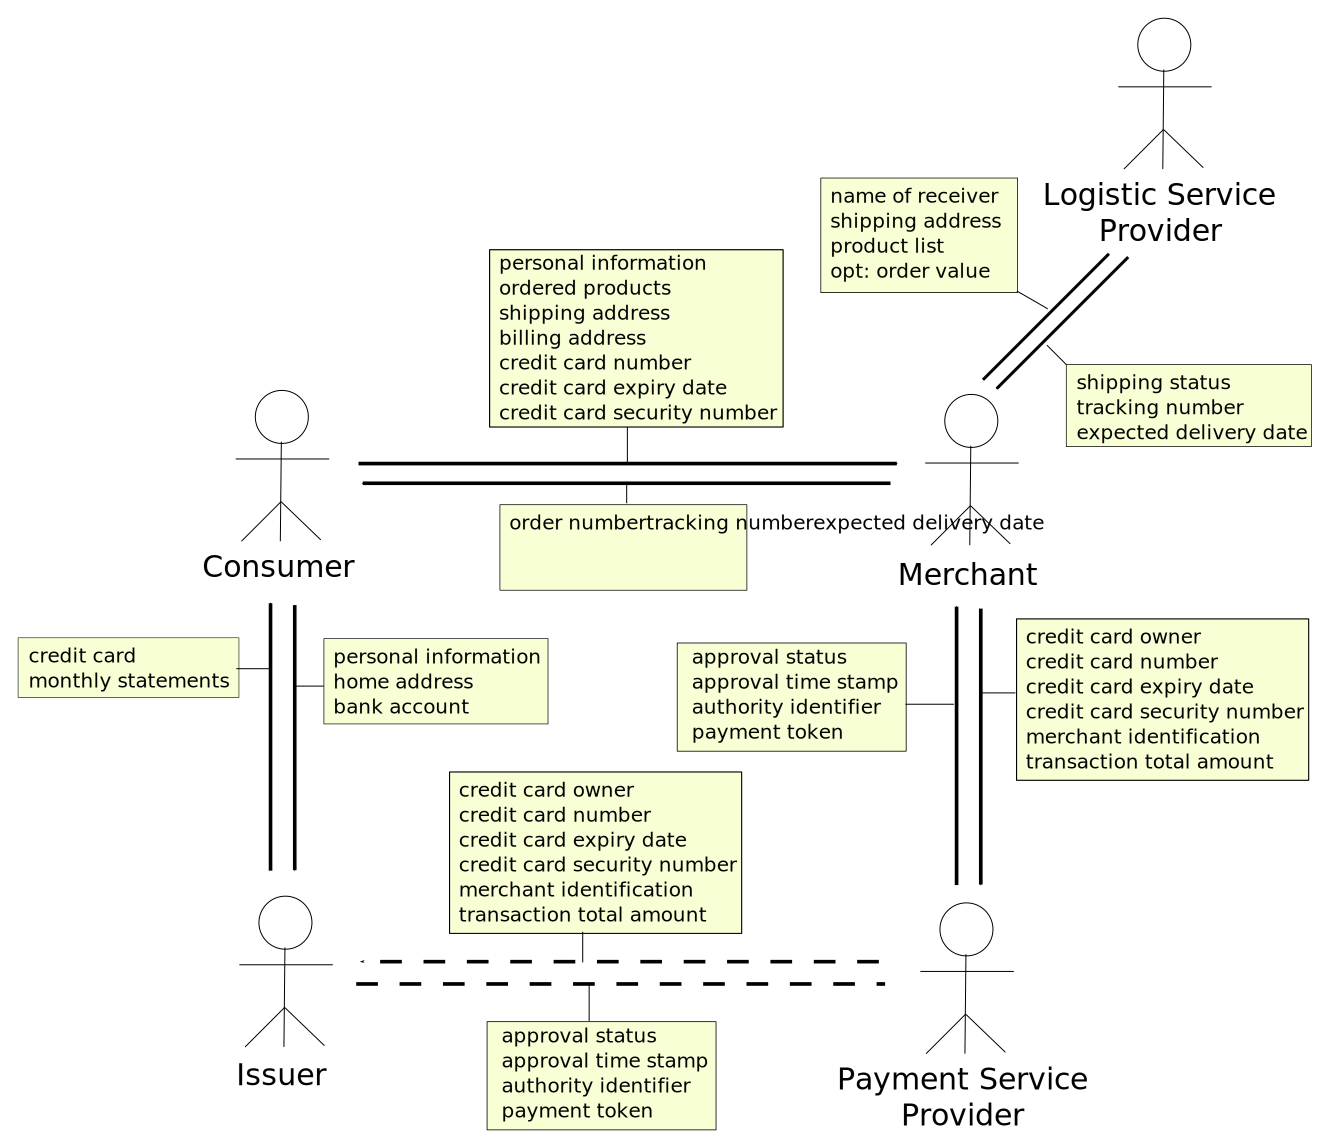
\includegraphics[width=0.9\columnwidth]{images/e-commerce-stakeholder.pdf}
	\caption{Stakeholders and data flow in \gls{E-commerce} scenario}
\label{fig:images_e_commerce_stakeholder}
\end{figure}


% sub chapter e-commerce fraud incidents
%!TEX root = ../MasterThesis.tex

\section{E-commerce fraud incidents}
\label{sec:scenario_fraud}

Based on the previous sections one can come up with strategies a fraudster might use to trick the E-commerce system. To do so the criminal will have to get access to credit card information in the first place. Therefore this section first looks into ways a criminal might get access to credit card and personal information in the E-commerce scenario. After that the section describes possible strategies a fraudster can use to trick the system. The section ends with a discussion of the E-commerce fraud incident handling as it is in place today.

\subsection{Credit Card data breaches}
\label{subsec:leaking_credit_cards}

 In the Section~\ref{sec:stakeholder_data_flow} one could already figure out the parties, who have access to or store credit card information in the E-commerce scenario, namely:\@

\begin{itemize}
  \item the consumer as owner of the credit card
  \item the issuing bank, who handed out the credit card to the consumer
  \item the merchant, if the consumer is paying with a credit card
  \item the Payment Service Provider, if the consumer is paying with a credit card online
\end{itemize}

The \gls{PSP} does receive the credit card information from the merchant during the authorization of the payment. If the \gls{PSP} does the authorization herself, she is also the participant, who stores and holds the credit card information in her backend databases. As mentioned earlier the \gls{PSP} should follow industry standards and guidelines for storing and processing payment-related information; especially the PCI/DSS standard \citep{virtue2009payment}. In addition she is responsible for monitoring her systems with an intrusion detection program. This will trigger a signal as soon as an hacker got access to the internal databases. In that case the \gls{PSP} can put the leaked credit card information on an internal blacklist, so that these cards could no longer be used for further payments online. Additionally she will have to send a message to the corresponding issuers, to which the \gls{PSP} generally maintains a strong business relationship. The issuer will inform the affected credit card owners and send out a credit card to each of them. Due to this procedure in place, one can assume that the safety and security of credit card handling at the \gls{PSP} can be guaranteed. \\

The merchant receives the credit card information during the checkout process from the consumer. The credit card information is transfered via the public Internet from the consumer to the merchant and could be a victim of a man-in-the-middle attack, in which the hacker is intercepting the communication between the consumer and the merchant with the objective to capture the personal and payment-related information from the data transmission stream. Therefore the merchant should offer the Web shop via a secure communication channel only. For that she can use industry standards such as TLS to encrypt the information send between both parties. This will make it more difficult for an attacker to get to the plaintext information exchanged between consumer and merchant during the checkout process. \\

As the merchant is not processing the credit card information directly, she also do not have to store them in her own backend databases. The merchant is asking the \gls{PSP} or issuer of the card for authorization of the credit card payment and receives an unique payment token in response, if the authorization was successful. As stated in the PCI/DSS standard \citep{virtue2009payment} a merchant should never store the whole credit card information in her databases, but should use this unique payment token and shortened credit card data (especially abbreviated credit card numbers) to refer to the specific payment later. Due to this procedure in place one can conclude, that breaking into the systems of a merchant will not result in any leaked credit card information, if the merchant follows these guidelines. \\

The issuer is a valuable target for hacking into the backend systems with the objective to leak a massive amount of credit card and owner information. As a financial institute the issuer have to follow a huge set of regulations and safety procedures to be able to participate on the market. It can be assumed that at least the same safety mechanisms are valid as are in place for the \gls{PSP}. This means constantly monitoring the internal systems with an intrusion detection mechanism and blacklisting any leaked credit card. In addition to the monitoring of all online activities (as also the \gls{PSP} does) the issuing bank can monitor activities done with the credit card in the offline world too. In case of suspicious activities the credit card can be blocked and a new one will be send out to the credit card owner. \\

The consumer is also a valuable target for eavesdropping on credit card and personal information. She is also the weakest and most unsecure party in the whole E-commerce scenario. As said above a lot of the protection mechanisms of the other participants are relying on implementing industry standards and on constantly monitoring the own systems for malicious activities. This can not be securely said about the computer of the consumer. Whether she is using up-to-date security programs (e.g.\ an Antivirus tool and a firewall) on her computer or not is out of reach of the others to verify. Additionally, a consumer can fall victim to a phishing attack, that will send her to a malicious Web site with the intend to get her personal information. In some seldom cases the consumer might cooperate with the fraudster, or might be the fraudster herself with the intend to trick the system for her self-interest. Due to this the E-commerce fraud investigation can not rely on information from the consumer, but instead has to figure out if the transaction in question was made from the real owner of the credit card or from a frauster.

% subsection leaking_credit_cards (end)

\subsection{E-commerce fraud strategies}
\label{subsec:strategies_fraudster}

After a fraudster has got access to leaked credit card information she can come up with the following strategies to trick the E-commerce system:\@

\begin{enumerate}
  \item a fraudster owns \textbf{one} leaked credit card information and try to use it for ordering products from \textbf{multiple} merchants on the Internet
  \item a fraudster owns \textbf{multiple} leaked credit card information and try to use them for ordering products from \textbf{one} merchant on the Internet
  \item a combination of the two cases mentioned before, that can also be related to as a series of the first fraud activity
\end{enumerate}

In the first scenario, in which the fraudster is trying out a leaked credit card for ordering products on Web shops of various merchants, each of the merchant only sees the transaction that takes place in her system. It will make it more difficult for the merchant to detect whether this is a fraud transaction or not, because she is not aware of the attempts the fraudster did on other merchant's Web shops. \\

As each merchant will rely on a \gls{PSP} or issuer to verify the credit card payment, it is in the responsibility of these participants to recognize fraud transactions in this scenario. To be able to do so, the \gls{PSP} and also the issuer are monitoring the usage of credit cards and are actively looking for suspicious activities. The fraud prevention mechanisms in place are mostly working on a rule-based, and in some cases also score-based systems running in the internal network of the \gls{PSP} and issuer. These systems are fed with the information the merchant sends with the payment authorization request and will come up with either:\@

\begin{enumerate}
  \item Yes, this looks like a fraudulent transaction and has to be blocked
  \item No, this seems to be a valid transaction and should be acknowledged
  \item Maybe, this transaction might be valid, but there is some uncertainty in the validation of it. These edge cases are routed to a human operator of the \gls{PSP} or issuer to decide on how to proceed with it
\end{enumerate}

As a recent study shows the success rate of the fraud prevention systems heavily relies on the techniques used to validate the transaction data \citep{rana2015survey}. The outcome is, that ca. 70 to 80 percent of the fraudulent transactions will be recognized as such and blocked successfully. That still means 20 to 30 percent of fraudulent transactions could not be recognized as such. For handling these cases the organisations employ special trained staff, that is operating 24/7 and 365 days a year, to be able to manage these edge cases. \\

As stated in the introduction of this Master thesis, there is a shift from the offline credit card fraud to the online world. This is also resembled in current figures of E-commerce fraud incidents, whose show that it makes up to 85 percent of all credit card fraud attempts and have on average a transaction value of 500 to 600 EURO.\\

As the \gls{PSP}s and the issuers do not have any order details, they can only decide on the information given during the authorization request (see Section~\ref{sec:stakeholder_analysis}). At most they can validate the branch the merchant is operating in, and it might come as no surprise that the fraudsters are regularly using Web shops of merchants, who offer either electronics, clothings, entertainment- or travel-related products. These are also the most commonly used sources of \textbf{\underline{valid}} E-commerce transactions, and will therefore make any fraudulent transaction very difficult to detect. \\

At the end it might be the owner of the credit card, who detects suspicious activities on her credit card account and informs the issuing bank about it. Based on current regulations and laws the issuing bank has to rollback the fraudulent transaction on request of the consumer, which means that the merchant will have to cover the costs of the E-commerce fraud (as she is not receiving the money for the products that has been already shipped to the fraudster). \\

Looking at the second scenario of the E-commerce fraud strategies at the beginning of this section, a merchant will receive multiple requests from a fraudster, who is trying out various leaked credit cards for finishing an order. This kind of E-commerce fraud can be recognized at the systems of the merchant due to the same source \gls{IP} address of the requests, or due to having the same shipping address for orders with different credit cards. Therefore, one can conclude that also merchants must take an active role in the fraud prevention process (if they do not already do so) and try to minimize the amount of fraudulent transactions taken place on their Web shops. As this scenario is likely be manageable with additional fraud prevention mechanisms at the merchant, and does not need to involve other parties of the E-commerce scenario to figure out the validity of the transaction, this second scenario falls out of scope of this Master thesis.

% subsection strategies_fraudster (end)

\subsection{E-commerce fraud incidents handling}
\label{subsec:e_commerce_fraud_handling}

If the fraud prevention systems at the \gls{PSP} or issuer are detecting a suspecious transaction, an operator working in a special department within the organisation will be informed about the transaction via a notification on his computer. This operator will have to decide whether the transaction looks valid and should be acknowledged, or seems to be fraudulent and has to be denied. To be able to decide this, she is going to look into the recent usages of the credit card in question. Whereas it will be easy to recognize that a credit card, that was just being used in a shop in Germany, could not be used in a shop in US or Asia within a short timeframe due to physical constraints in the real world, the same consumer can order products from an US or Asian online retailer with ease within minutes. So these initial geographical contraints, that work well with real world usage patterns of credit cards (a fraud prevention mechanism called geo-fencing), will no longer work well in the E-commerce scenario. \\

So the operator has to found her decision on the transaction information at hand. Initially she can check for the amount that has been paid with the credit card. One can assume that small amounts will be covered by the \gls{PSP} or issuer, who will take over the risk for a false authorization. But with an increased value of the items ordered, the \gls{PSP} or issuer is putting back the risk to the merchant in case of customer complaints later. At a second glance the operator can verify whether the consumer has had any business relationship with the merchant in the past or not as well as verify the retail branch the merchant operates in. Although these are weak hints for investigating the validity of an E-commerce transaction as they can be bypassed by the fraudster with ease (see above). \\

To make a solid decision the operator will have to get in contact with the merchants the credit card has been used with recently, and have to ask for additional information such as:\@

\begin{itemize}
  \item does the consumer owns an user account with the Web shop?
  \item what is the consumer usually looking for in the Web shop?
  \item does the shipping address matches the billing address for the order?
  \item if not, has the user send products to this shipping address in the past?
  \item what has been ordered, incl.\ detailed product information such as brand, model, product categories, \ldots
\end{itemize}

In some cases the \gls{PSP} or issuer might have had a business relationship with the online merchant in the past. So the \gls{PSP} or issuer might already know whom to contact from the support personnel of the merchant. But in most cases the contact person might not be known to the \gls{PSP} or issuer resulting in sending a request to the general support staff via the contact formulars on the merchants Web site. \\

Getting the right information might take time as the correct addressee from the support department of the merchant is unknown, the merchant do not have specialized staff at hand to handle these kind of issues, or there are misunderstandings on handling the case due to language barriers or different incentives between the participants. Additionally the operator have to collect the available information from these merchants, note them down and try to build a ``picture'' out of it. In case the initial information received from one of the participants have not been enough, she will have to get in contact with the support personnel again. Due to this getting an in-depth overview of a suspecious transaction is likely taking hours if not days or weeks. That is definetly way to much time and effort to look into any of these transactions. Therefore one can assume that this detailed analysis of any suspecious transaction will not take place today, instead most of these transactions will be acknowledged without doubt after a first short look and plausibility check. \\

Still the merchants as well as the \gls{PSP} and issuer have a high incentive for keeping the success rates and numbers of any fraudulent activity low. For the \gls{PSP} and issuing bank there are regulations stating that at maximum only 1 thousands of the overall transactions should be fraudulent (note: numbers stated are valid for the EU). This keeps the pressure on these financial instituts to invest in fraud prevention techniques for being able to stay in business. For the merchant it is of high interest that a fraudulent transaction can be resolved, before the fraudster receives the ordered products. In the worst case scenario just one successfully performed fraudulent transaction in an E-commerce shop will trigger hundreds if not thousands of following attempts from other fraudsters, as past experiences have shown. \\

% subsection e_commerce_fraud_handling

% section scenario_fraud (end)


% sub chapter scope of thesis
%!TEX root = ../MasterThesis.tex

\section{Scope of this Master Thesis}
\label{sec:scope_thesis}

As laid out in the previous section, the most interesting \gls{E-commerce} fraud scenario is the one, in which fraudsters use leaked credit card information to order products or services from various merchants on the Internet. This is currently most likely to be successful, because there is a lack of information on the side of the merchants as well as the \gls{PSP}s and the issuers. Each of the affected merchants just noticed the transaction that takes place in their own Web shop, without knowing about the other attempts the fraudsters do on the Internet. The \gls{PSP}s and the issuers will both notice the active use of a credit card on different Web shops though, but do not have any transaction details. Therefore they could not correlate the data from these transactions to check for suspicious activities. \\

Based on the current credit card usage patterns of the fraudsters, who will try a leaked credit card in commonly used Web shops, it is more likely that these fraudulent transactions will not be recognized on time by the existing fraud prevention techniques in place. \\

A simple approach to solve these issues would be to just share more information of the ongoing transactions between the merchants, the \gls{PSP}s and the issuers. This approach might be subject to fail though, because adapting and harmonizing the communication interfaces between the Web shops from various online merchants and the Web Service interfaces of different \gls{PSP}s and issuers are an enormous undertaking. Any attempt will likely not succeed due to different notions of the communication patterns and data structures exchanged between all relevant participants. \\

To solve these problems this Master thesis will look into the information sharing issues in detail and try to come up with a solution to answer the most important question of this scenario: \@

\begin{quotation}
  \textit{Is this transaction really a valid \gls{E-commerce} transaction?}
\end{quotation}

Looking into the stakeholders, who can provide useful information to decide it, one will come up with:\@

\begin{enumerate}
    \item \textbf{Merchants}, who can provide additional information of each \gls{E-commerce} transaction in question.
    \item \textbf{\gls{PSP}s/issuers}, who have information about the credit card usage patterns and the original credit card owners.
    \item \textbf{\gls{LSP}s}, who can offer information about whether an order has already been shipped or not, and in the former case to whom it has been handed over.
\end{enumerate}

Its important to point out that parts of the shared information are confidential or business-critical to at least one of the stakeholders involved. Due to this fact the data sharing has to be secured, and access to the resources has to be granted to selected participants of the scenario only. This Master thesis will focus on the data sharing, collecting and combining aspects of the collaborative system. A detailed discussion of the security aspects of it, \gls{incl}\ how to restrict access to the data with available techniques such as \gls{OAuth}, is out of scope of the thesis though.\\

Additionally, as a \gls{CSCW} system \emph{always} consists of a social and a technological component introducing such a collaborative system into an existing organization will raise issues of user acceptance and adaptation to business processes that are (due to time and space constraints) also left out of the discussions in this Master thesis.

% section scope_thesis (end)


% chapter context analysis (end)
